% !TeX encoding = UTF-8
% !TeX program = xelatex
% !TeX spellcheck = en_US

\documentclass[degree=bachelor]{thuthesis}
  % 学位 degree:
  %   doctor | master | bachelor | postdoc
  % 学位类型 degree-type:
  %   academic(默认)| professional
  % 语言 language
  %   chinese(默认)| english
  % 字体库 fontset
  %   windows | mac | fandol | ubuntu
  % 建议终版使用 Windows 平台的字体编译


% 论文基本配置,加载宏包等全局配置
% !TeX root = ./__ylc_main.tex

% 论文基本信息配置

\thusetup{
  %******************************
  % 注意:
  %   1. 配置里面不要出现空行
  %   2. 不需要的配置信息可以删除
  %   3. 建议先阅读文档中所有关于选项的说明
  %******************************
  %
  % 输出格式
  %   选择打印版(print)或用于提交的电子版(electronic),前者会插入空白页以便直接双面打印
  %
  output = print,
  % 格式类型
  %   默认为论文(thesis),也可以设置为开题报告(proposal)
  % thesis-type = proposal,
  %
  % 标题
  %   可使用“\\”命令手动控制换行
  %
  title  = {清华大学-学位论文 \LaTeX{} 模板\\使用示例文档 v\version},
  title* = {An Introduction to \LaTeX{} Thesis Template of Tsinghua
            University v\version},
  %
  % 学科门类
  %   1. 学术型
  %      - 中文
  %        需注明所属的学科门类,例如:
  %        哲学、经济学、法学、教育学、文学、历史学、理学、工学、农学、医学、
  %        军事学、管理学、艺术学
  %      - 英文
  %        博士:Doctor of Philosophy
  %        硕士:
  %          哲学、文学、历史学、法学、教育学、艺术学门类,公共管理学科
  %          填写“Master of Arts“,其它填写“Master of Science”
  %   2. 专业型
  %      直接填写专业学位的名称,例如:
  %      教育博士、工程硕士等
  %      Doctor of Education, Master of Engineering
  %   3. 本科生不需要填写
  %
  degree-category  = {工学硕士},
  degree-category* = {Master of Science},
  %
  % 培养单位
  %   填写所属院系的全名
  %
  department = {计算机科学与技术系},
  %
  % 学科
  %   1. 研究生学术型学位,获得一级学科授权的学科填写一级学科名称,其他填写二级学科名称
  %   2. 本科生填写专业名称,第二学位论文需标注“(第二学位)”
  %
  discipline  = {计算机科学与技术},
  discipline* = {Computer Science and Technology},
  %
  % 专业领域
  %   1. 设置专业领域的专业学位类别,填写相应专业领域名称
  %   2. 2019 级及之前工程硕士学位论文,在 `engineering-field` 填写相应工程领域名称
  %   3. 其他专业学位类别的学位论文无需此信息
  %
  % professional-field  = {计算机技术},
  % professional-field* = {Computer Technology},
  %
  % 姓名
  %
  author  = {薛瑞尼},
  author* = {Xue Ruini},
  %
  % 学号
  % 仅当书写开题报告时需要(同时设置 `thesis-type = proposal')
  %
  % student-id = {2000310000},
  %
  % 指导教师
  %   中文姓名和职称之间以英文逗号“,”分开,下同
  %
  supervisor  = {郑纬民, 教授},
  supervisor* = {Professor Zheng Weimin},
  %
  % 副指导教师
  %
  associate-supervisor  = {陈文光, 教授},
  associate-supervisor* = {Professor Chen Wenguang},
  %
  % 联合指导教师
  %
  % co-supervisor  = {某某某, 教授},
  % co-supervisor* = {Professor Mou Moumou},
  %
  % 日期
  %   使用 ISO 格式;默认为当前时间
  %
  % date = {2019-07-07},
  %
  % 是否在中文封面后的空白页生成书脊(默认 false)
  %
  include-spine = false,
  %
  % 密级和年限
  %   秘密, 机密, 绝密
  %
  % secret-level = {秘密},
  % secret-year  = {10},
  %
  % 博士后专有部分
  %
  % clc                = {分类号},
  % udc                = {UDC},
  % id                 = {编号},
  % discipline-level-1 = {计算机科学与技术},  % 流动站(一级学科)名称
  % discipline-level-2 = {系统结构},          % 专业(二级学科)名称
  % start-date         = {2011-07-01},        % 研究工作起始时间
}

% 载入所需的宏包

% 定理类环境宏包
\usepackage{amsthm}
% 也可以使用 ntheorem
% \usepackage[amsmath,thmmarks,hyperref]{ntheorem}

\thusetup{
  %
  % 数学字体
  % math-style = GB,  % GB | ISO | TeX
  math-font  = xits,  % stix | xits | libertinus
}

% 可以使用 nomencl 生成符号和缩略语说明
% \usepackage{nomencl}
% \makenomenclature

% 表格加脚注
\usepackage{threeparttable}

% 表格中支持跨行
\usepackage{multirow}

% 固定宽度的表格。
% \usepackage{tabularx}

% 跨页表格
\usepackage{longtable}

% 算法
\usepackage{algorithm}
\usepackage{algorithmic}

% 量和单位
\usepackage{siunitx}

% 参考文献使用 BibTeX + natbib 宏包
% 顺序编码制
\usepackage[sort]{natbib}
\bibliographystyle{thuthesis-numeric}

% 著者-出版年制
% \usepackage{natbib}
% \bibliographystyle{thuthesis-author-year}

% 生命科学学院要求使用 Cell 参考文献格式(2023 年以前使用 author-date 格式)
% \usepackage{natbib}
% \bibliographystyle{cell}

% 本科生参考文献的著录格式
% \usepackage[sort]{natbib}
% \bibliographystyle{thuthesis-bachelor}

% 参考文献使用 BibLaTeX 宏包
% \usepackage[style=thuthesis-numeric]{biblatex}
% \usepackage[style=thuthesis-author-year]{biblatex}
% \usepackage[style=gb7714-2015]{biblatex}
% \usepackage[style=apa]{biblatex}
% \usepackage[style=mla-new]{biblatex}
% 声明 BibLaTeX 的数据库
% \addbibresource{ref/refs.bib}

% 定义所有的图片文件在 figures 子目录下
\graphicspath{{figures/}}

% 数学命令
\makeatletter
\newcommand\dif{%  % 微分符号
  \mathop{}\!%
  \ifthu@math@style@TeX
    d%
  \else
    \mathrm{d}%
  \fi
}
\makeatother

% hyperref 宏包在最后调用
\usepackage{hyperref}



\begin{document}

% 封面
\maketitle

% 学位论文指导小组、公开评阅人和答辩委员会名单
% 本科生不需要
% !TeX root = ../thuthesis-example.tex

\begin{committee}[name={学位论文指导小组、公开评阅人和答辩委员会名单}]

  \newcolumntype{C}[1]{@{}>{\centering\arraybackslash}p{#1}}

  \section*{指导小组名单}

  \begin{center}
    \begin{tabular}{C{3cm}C{3cm}C{9cm}@{}}
      李XX & 教授     & 清华大学 \\
      王XX & 副教授   & 清华大学 \\
      张XX & 助理教授 & 清华大学 \\
    \end{tabular}
  \end{center}


  \section*{公开评阅人名单}

  \begin{center}
    \begin{tabular}{C{3cm}C{3cm}C{9cm}@{}}
      刘XX & 教授   & 清华大学                    \\
      陈XX & 副教授 & XXXX大学                    \\
      杨XX & 研究员 & 中国XXXX科学院XXXXXXX研究所 \\
    \end{tabular}
  \end{center}


  \section*{答辩委员会名单}

  \begin{center}
    \begin{tabular}{C{2.75cm}C{2.98cm}C{4.63cm}C{4.63cm}@{}}
      主席 & 赵XX                  & 教授                    & 清华大学       \\
      委员 & 刘XX                  & 教授                    & 清华大学       \\
          & \multirow{2}{*}{杨XX} & \multirow{2}{*}{研究员} & 中国XXXX科学院 \\
          &                       &                         & XXXXXXX研究所  \\
          & 黄XX                  & 教授                    & XXXX大学       \\
          & 周XX                  & 副教授                  & XXXX大学       \\
      秘书 & 吴XX                  & 助理研究员              & 清华大学       \\
    \end{tabular}
  \end{center}

\end{committee}



% 也可以导入 Word 版转的 PDF 文件
% \begin{committee}[file=figures/committee.pdf]
% \end{committee}


% 使用授权的说明
% 本科生开题报告不需要
\copyrightpage
% 将签字扫描后授权文件 scan-copyright.pdf 替换原始页面
% \copyrightpage[file=scan-copyright.pdf]

\frontmatter
% !TeX root = ../__ylc_main.tex

% title = {基于解题过程的学生思维能力评估},

% 中英文摘要和关键字

\begin{abstract}
  传统教学中,学生在完成解题之后由老师统一批改,欠缺了对其过程中的思路的跟踪。人工批改作业费时费力,如果要去挖掘每一个学生解题过程的思路细节,更加繁琐和复杂,不可能做到很细致。

  近年来大语言模型(LLM)的发展成熟,为解决这一问题提供了新的思路。LLM已经具有强大的自然语言理解能力,可以自动化地解析和跟踪学生的解题过程。本研究提出了一种基于LLM的学生思维能力评估方法,通过对解题过程中思路的详细建模,从而评估学生的思维能力。在思路建模的基础上,本研究还实现了解题过程的错因分析,对于学生可以准确地指出发生错误的步骤,对于老师可以获得班级学生的错因统计。

  本研究使用安卓平台采集数据,分别使用数位板和设备摄像头收集解题过程的笔迹信息、视频和音频信息。然后在 LLM 的辅助下完成解题过程的思路建模和错因分析。

  本研究是将 LLM 应用于教育领域来进行思维建模的首次尝试,实验结果表明,该方法可以有效地评估学生的思维能力,为自动化题目讲解以及在中学的大规模应用提供了基础。

  % 关键词用“英文逗号”分隔,输出时会自动处理为正确的分隔符
  \thusetup{
    keywords = {思维建模, 大语言模型, 解题过程分析, 人机交互},
  }
\end{abstract}

\begin{abstract*}
  % English abstract, translation of above Chinese abstract

  In traditional teaching, students' ideas are not tracked in the process of solving problems. Manual correction of homework is time-consuming and laborious. It is more cumbersome and complex to dig into the details of the thinking process of each student, and it is impossible to be very meticulous.

  In recent years, the development of large language models (LLM) has matured, providing new ideas to solve this problem. LLM already has powerful natural language understanding capabilities and can automatically parse and track students' problem-solving processes. This study proposes a method for evaluating students' thinking ability based on LLM, which evaluates students' thinking ability by modeling the details of their thinking process. Based on the modeling of ideas, this study also implements the analysis of the causes of errors in the problem-solving process, which can accurately point out the steps where students make mistakes and provide teachers with statistics on the causes of errors in the class.

  This study collects data on the Android platform, using a graphics tablet and device camera to collect handwriting information, video, and audio information during the problem-solving process. Then, with the assistance of LLM, the thinking process modeling and error analysis of the problem-solving process are completed.

  This study is the first attempt to apply LLM to the field of education for thinking modeling. The experimental results show that this method can effectively evaluate students' thinking ability, providing a foundation for automated problem explanation and large-scale application in secondary schools.

  % Use comma as separator when inputting
  \thusetup{
    keywords* = {Thinking Modeling, Large Language Model, Problem Solving Process Analysis, Human-Computer Interaction},
  }
\end{abstract*}


% 目录
\tableofcontents

% 插图和附表清单
% 本科生的插图索引和表格索引需要移至正文之后、参考文献前
% \listoffiguresandtables  % 插图和附表清单(仅限研究生)
\listoffigures           % 插图清单
\listoftables            % 附表清单

% 符号对照表
% !TeX root = ../__ylc_main.tex

\begin{denotation}[3cm]
  \item[PI] 聚酰亚胺
  \item[MPI] 聚酰亚胺模型化合物,N-苯基邻苯酰亚胺
  \item[PBI] 聚苯并咪唑
  \item[MPBI] 聚苯并咪唑模型化合物,N-苯基苯并咪唑
  \item[PY] 聚吡咙
  \item[PMDA-BDA] 均苯四酸二酐与联苯四胺合成的聚吡咙薄膜
  \item[MPY] 聚吡咙模型化合物
  \item[As-PPT] 聚苯基不对称三嗪
  \item[MAsPPT] 聚苯基不对称三嗪单模型化合物,3,5,6-三苯基-1,2,4-三嗪
  \item[DMAsPPT] 聚苯基不对称三嗪双模型化合物(水解实验模型化合物)
  \item[S-PPT] 聚苯基对称三嗪
  \item[MSPPT] 聚苯基对称三嗪模型化合物,2,4,6-三苯基-1,3,5-三嗪
  \item[PPQ] 聚苯基喹噁啉
  \item[MPPQ] 聚苯基喹噁啉模型化合物,3,4-二苯基苯并二嗪
  \item[HMPI] 聚酰亚胺模型化合物的质子化产物
  \item[HMPY] 聚吡咙模型化合物的质子化产物
  \item[HMPBI] 聚苯并咪唑模型化合物的质子化产物
  \item[HMAsPPT] 聚苯基不对称三嗪模型化合物的质子化产物
  \item[HMSPPT] 聚苯基对称三嗪模型化合物的质子化产物
  \item[HMPPQ] 聚苯基喹噁啉模型化合物的质子化产物
  \item[PDT] 热分解温度
  \item[HPLC] 高效液相色谱(High Performance Liquid Chromatography)
  \item[HPCE] 高效毛细管电泳色谱(High Performance Capillary lectrophoresis)
  \item[LC-MS] 液相色谱-质谱联用(Liquid chromatography-Mass Spectrum)
  \item[TIC] 总离子浓度(Total Ion Content)
  \item[\textit{ab initio}] 基于第一原理的量子化学计算方法,常称从头算法
  \item[DFT] 密度泛函理论(Density Functional Theory)
  \item[$E_a$] 化学反应的活化能(Activation Energy)
  \item[ZPE] 零点振动能(Zero Vibration Energy)
  \item[PES] 势能面(Potential Energy Surface)
  \item[TS] 过渡态(Transition State)
  \item[TST] 过渡态理论(Transition State Theory)
  \item[$\increment G^\neq$] 活化自由能(Activation Free Energy)
  \item[$\kappa$] 传输系数(Transmission Coefficient)
  \item[IRC] 内禀反应坐标(Intrinsic Reaction Coordinates)
  \item[$\nu_i$] 虚频(Imaginary Frequency)
  \item[ONIOM] 分层算法(Our own N-layered Integrated molecular Orbital and molecular Mechanics)
  \item[SCF] 自洽场(Self-Consistent Field)
  \item[SCRF] 自洽反应场(Self-Consistent Reaction Field)
\end{denotation}



% 也可以使用 nomencl 宏包,需要在导言区
% \usepackage{nomencl}
% \makenomenclature

% 在这里输出符号说明
% \printnomenclature[3cm]

% 在正文中的任意为都可以标题
% \nomenclature{PI}{聚酰亚胺}
% \nomenclature{MPI}{聚酰亚胺模型化合物,N-苯基邻苯酰亚胺}
% \nomenclature{PBI}{聚苯并咪唑}
% \nomenclature{MPBI}{聚苯并咪唑模型化合物,N-苯基苯并咪唑}
% \nomenclature{PY}{聚吡咙}
% \nomenclature{PMDA-BDA}{均苯四酸二酐与联苯四胺合成的聚吡咙薄膜}
% \nomenclature{MPY}{聚吡咙模型化合物}
% \nomenclature{As-PPT}{聚苯基不对称三嗪}
% \nomenclature{MAsPPT}{聚苯基不对称三嗪单模型化合物,3,5,6-三苯基-1,2,4-三嗪}
% \nomenclature{DMAsPPT}{聚苯基不对称三嗪双模型化合物(水解实验模型化合物)}
% \nomenclature{S-PPT}{聚苯基对称三嗪}
% \nomenclature{MSPPT}{聚苯基对称三嗪模型化合物,2,4,6-三苯基-1,3,5-三嗪}
% \nomenclature{PPQ}{聚苯基喹噁啉}
% \nomenclature{MPPQ}{聚苯基喹噁啉模型化合物,3,4-二苯基苯并二嗪}
% \nomenclature{HMPI}{聚酰亚胺模型化合物的质子化产物}
% \nomenclature{HMPY}{聚吡咙模型化合物的质子化产物}
% \nomenclature{HMPBI}{聚苯并咪唑模型化合物的质子化产物}
% \nomenclature{HMAsPPT}{聚苯基不对称三嗪模型化合物的质子化产物}
% \nomenclature{HMSPPT}{聚苯基对称三嗪模型化合物的质子化产物}
% \nomenclature{HMPPQ}{聚苯基喹噁啉模型化合物的质子化产物}
% \nomenclature{PDT}{热分解温度}
% \nomenclature{HPLC}{高效液相色谱(High Performance Liquid Chromatography)}
% \nomenclature{HPCE}{高效毛细管电泳色谱(High Performance Capillary lectrophoresis)}
% \nomenclature{LC-MS}{液相色谱-质谱联用(Liquid chromatography-Mass Spectrum)}
% \nomenclature{TIC}{总离子浓度(Total Ion Content)}
% \nomenclature{\textit{ab initio}}{基于第一原理的量子化学计算方法,常称从头算法}
% \nomenclature{DFT}{密度泛函理论(Density Functional Theory)}
% \nomenclature{$E_a$}{化学反应的活化能(Activation Energy)}
% \nomenclature{ZPE}{零点振动能(Zero Vibration Energy)}
% \nomenclature{PES}{势能面(Potential Energy Surface)}
% \nomenclature{TS}{过渡态(Transition State)}
% \nomenclature{TST}{过渡态理论(Transition State Theory)}
% \nomenclature{$\increment G^\neq$}{活化自由能(Activation Free Energy)}
% \nomenclature{$\kappa$}{传输系数(Transmission Coefficient)}
% \nomenclature{IRC}{内禀反应坐标(Intrinsic Reaction Coordinates)}
% \nomenclature{$\nu_i$}{虚频(Imaginary Frequency)}
% \nomenclature{ONIOM}{分层算法(Our own N-layered Integrated molecular Orbital and molecular Mechanics)}
% \nomenclature{SCF}{自洽场(Self-Consistent Field)}
% \nomenclature{SCRF}{自洽反应场(Self-Consistent Reaction Field)}



% 正文部分
\mainmatter
% !TeX root = ../thuthesis-example.tex

\chapter{论文主要部分的写法}

研究生学位论文撰写,除表达形式上需要符合一定的格式要求外,内容方面上也要遵循一些共性原则。

通常研究生学位论文只能有一个主题(不能是几块工作拼凑在一起),该主题应针对某学科领域中的一个具体问题展开深入、系统的研究,并得出有价值的研究结论。
学位论文的研究主题切忌过大,例如,“中国国有企业改制问题研究”这样的研究主题过大,因为“国企改制”涉及的问题范围太广,很难在一本研究生学位论文中完全研究透彻。



\section{论文的语言及表述}

除国际研究生外,学位论文一律须用汉语书写。
学位论文应当用规范汉字进行撰写,除古汉语研究中涉及的古文字和参考文献中引用的外文文献之外,均采用简体汉字撰写。

国际研究生一般应以中文或英文书写学位论文,格式要求同上。
论文须用中文封面。

研究生学位论文是学术作品,因此其表述要严谨简明,重点突出,专业常识应简写或不写,做到立论正确、数据可靠、说明透彻、推理严谨、文字凝练、层次分明,避免使用文学性质的或带感情色彩的非学术性语言。

论文中如出现一个非通用性的新名词、新术语或新概念,需随即解释清楚。



\section{论文题目的写法}

论文题目应简明扼要地反映论文工作的主要内容,力求精炼、准确,切忌笼统。
论文题目是对研究对象的准确、具体描述,一般要在一定程度上体现研究结论,因此,论文题目不仅应告诉读者这本论文研究了什么问题,更要告诉读者这个研究得出的结论。
例如:“在事实与虚构之间:梅乐、卡彭特、沃尔夫的新闻观”就比“三个美国作家的新闻观研究”更专业、更准确。



\section{摘要的写法}

论文摘要是对论文研究内容的高度概括,应具有独立性和自含性,即应是 一篇简短但意义完整的文章。
通过阅读论文摘要,读者应该能够对论文的研究 方法及结论有一个整体性的了解,因此摘要的写法应力求精确简明。
论文摘要 应包括对问题及研究目的的描述、对使用的方法和研究过程进行的简要介绍、 对研究结论的高度凝练等,重点是结果和结论。

论文摘要切忌写成全文的提纲,尤其要避免“第 1 章……;第 2 章……;……”这样的陈述方式。



\section{引言的写法}

一篇学位论文的引言大致包含如下几个部分:
1、问题的提出;
2、选题背 景及意义;
3、文献综述;
4、研究方法;
5、论文结构安排。
\begin{itemize}
  \item 问题的提出:要清晰地阐述所要研究的问题“是什么”。
    \footnote{选题时切记要有“问题意识”,不要选不是问题的问题来研究。}
  \item 选题背景及意义:论述清楚为什么选择这个题目来研究,即阐述该研究对学科发展的贡献、对国计民生的理论与现实意义等。
  \item 文献综述:对本研究主题范围内的文献进行详尽的综合述评,“述”的同时一定要有“评”,指出现有研究状态,仍存在哪些尚待解决的问题,讲出自己的研究有哪些探索性内容。
  \item 研究方法:讲清论文所使用的学术研究方法。
  \item 论文结构安排:介绍本论文的写作结构安排。
\end{itemize}



\section{正文的写法}

本部分是论文作者的研究内容,不能将他人研究成果不加区分地掺和进来。
已经在引言的文献综述部分讲过的内容,这里不需要再重复。
各章之间要存在有机联系,符合逻辑顺序。



\section{结论的写法}

结论是对论文主要研究结果、论点的提炼与概括,应精炼、准确、完整,使读者看后能全面了解论文的意义、目的和工作内容。
结论是最终的、总体的结论,不是正文各章小结的简单重复。
结论应包括论文的核心观点,主要阐述作者的创造性工作及所取得的研究成果在本领域中的地位、作用和意义,交代研究工作的局限,提出未来工作的意见或建议。
同时,要严格区分自己取得的成果与指导教师及他人的学术成果。

在评价自己的研究工作成果时,要实事求是,除非有足够的证据表明自己的研究是“首次”、“领先”、“填补空白”的,否则应避免使用这些或类似词语。

% !TeX root = ../__ylc_main.tex

\chapter{相关研究综述}

本章从三个方面来介绍关于学生的认知建模以及大语言模型在此方面的应用的研究背景。第一部分介绍了学生认知建模的相关研究,包括知识追踪、认知诊断等方面。第二部分介绍了大语言模型的相关研究,包括大语言模型的基本原理、发展历程等。第三部分介绍了大语言模型在教育领域的应用,包括大语言模型在教育领域的应用前景、研究进展等。

\section{知识追踪和认知诊断}

随着信息技术的发展,人们逐渐开始探究如何用计算机来辅助教学,提高教学效率。在近几年大语言模型出现之前,人们就已经在使用传统的统计、机器学习,乃至近期的深度学习模型来试图刻画学生的知识掌握情况、对学生能力进行建模,并对学生未来的表现进行预测。知识追踪(Knowledge Tracing,KT)和认知诊断(Cognitive Diagnosis, CD)是这方面的两个重要研究方向。它们旨在通过对学生的学习过程和认知状态进行建模和分析,为教师提供个性化的教学支持和指导。

这两类工作都基于固定的题库和固定的知识点划分。知识追踪 的主要任务是根据学生的解题历史预测他们正确回答其他问题的可能性;认知诊断 的主要任务是根据学生的解题历史评估他们对各个知识点的掌握情况。

\subsection{知识追踪}

人类通过教学来传授知识的能力是人类智能的重要方面之一。人类教师可以通过观察学生的知识掌握情况,根据学生的需求定制教学。随着在线教育平台的兴起,机器也同样需要追踪学生的知识,为他们量身定制学习体验。这类研究问题被称为知识追踪(KT)问题。有效解决知识追踪问题将开发计算机辅助教育应用的潜力,为智能辅导系统、课程学习和学习材料推荐等智能教育系统提供算法解决方案。此外,从更广泛的角度来看, 知识追踪问题中所关注的“学生”可以是任何类型的智能体,包括人类和人工智能 Agent。因此,KT 的潜力可以推广到任何寻求为智能(如机器学习模型)定制学习体验的机器教学应用场景\cite{abdelrahman2023knowledge}。KT对在线学习系统和学生都具有重要意义。首先,KT模型能够开发个性化的自适应学习系统。一旦掌握了学生的知识状态,学习系统就可以为不同的学生定制更合适的学习方案,从而可以根据学生的熟练程度进行教学。其次,学生自己也可以更好地了解他们的学习过程,并逐渐更多地关注掌握不熟练的技能\cite{liu2019exploiting}。

知识追踪(Knowledge Tracing,KT)基于对学生行为序列的建模来获取学生的认知状态并预测学生未来的学习表现。知识追踪任务旨在根据学生的历史学习行为,实时地建模学生的知识状态,从而预测学生未来的学习成绩。

知识追踪已经研究了几十年,早期与KT相关的研究可以追溯到20世纪70年代末;但是\citet{corbett1994knowledge} 的工作是第一个引入“知识追踪”这一概念的研究,他们利用贝叶斯网络来模拟学生学习过程,这被称为贝叶斯知识追踪。随后越来越多的研究者开始关注与知识追踪相关的研究。例如,许多逻辑模型已被应用于KT,包括学习因子分析(Learning Factor Analysis)和表现因素分析(Performance Factor Analysis)。近年来,深度学习逐渐被应用与对KT任务的研究,因为它具有强大的提取和表示特征的能力,以及发现复杂结构的能力。例如,深度知识追踪引入了循环神经网络(RNN)进入KT任务,并被发现明显优于以前的方法。之后,通过考虑学习序列的各种特征,更多的方法将各种类型的神经网络引入到KT任务中。此外,由于实际应用的要求,KT模型的许多变体也不断开发,KT已经广泛应用于许多教育场景\cite{liu2021survey}。

\subsection{认知诊断}

在智能教育系统领域,认知诊断(Cognitive Diagnosis, CD)\cite{liu2023new}是一项基本而重要的任务,其目的是通过学生表现评估预测过程来衡量学生对特定知识概念的掌握程度。认知诊断有很多可能的应用,包括计算机自适应测试、定向培训和练习题目推荐系统。认知诊断系统一般都涉及一个题目-概念矩阵(也被称为 Q-矩阵),Q-矩阵经过专家的标注,用来表示每一道练习题中涉及到了哪些知识、概念或能力。多数认知诊断模型大多依赖于由领域专家标注的标记完全的 Q-矩阵来训练模型,这些研究侧重于增强响应记录的挖掘过程,以获得更好的诊断结果。

一个典型的认知诊断过程如图\ref{fig:cd_example}中例子所示。例如,在练习题目 v3 中考察了知识概念 k3 和 k5。根据 CD 模型的诊断,学生 u2 对这两个概念的熟练程度高于 u1,因为 u2 在练习题中回答正确,而 u1 回答错误。很明显,全标注 Q 矩阵在 CD 模型的可解释性(即诊断报告)方面起着至关重要的作用\cite{chen2024disentangling}。

\begin{figure}
    \centering
    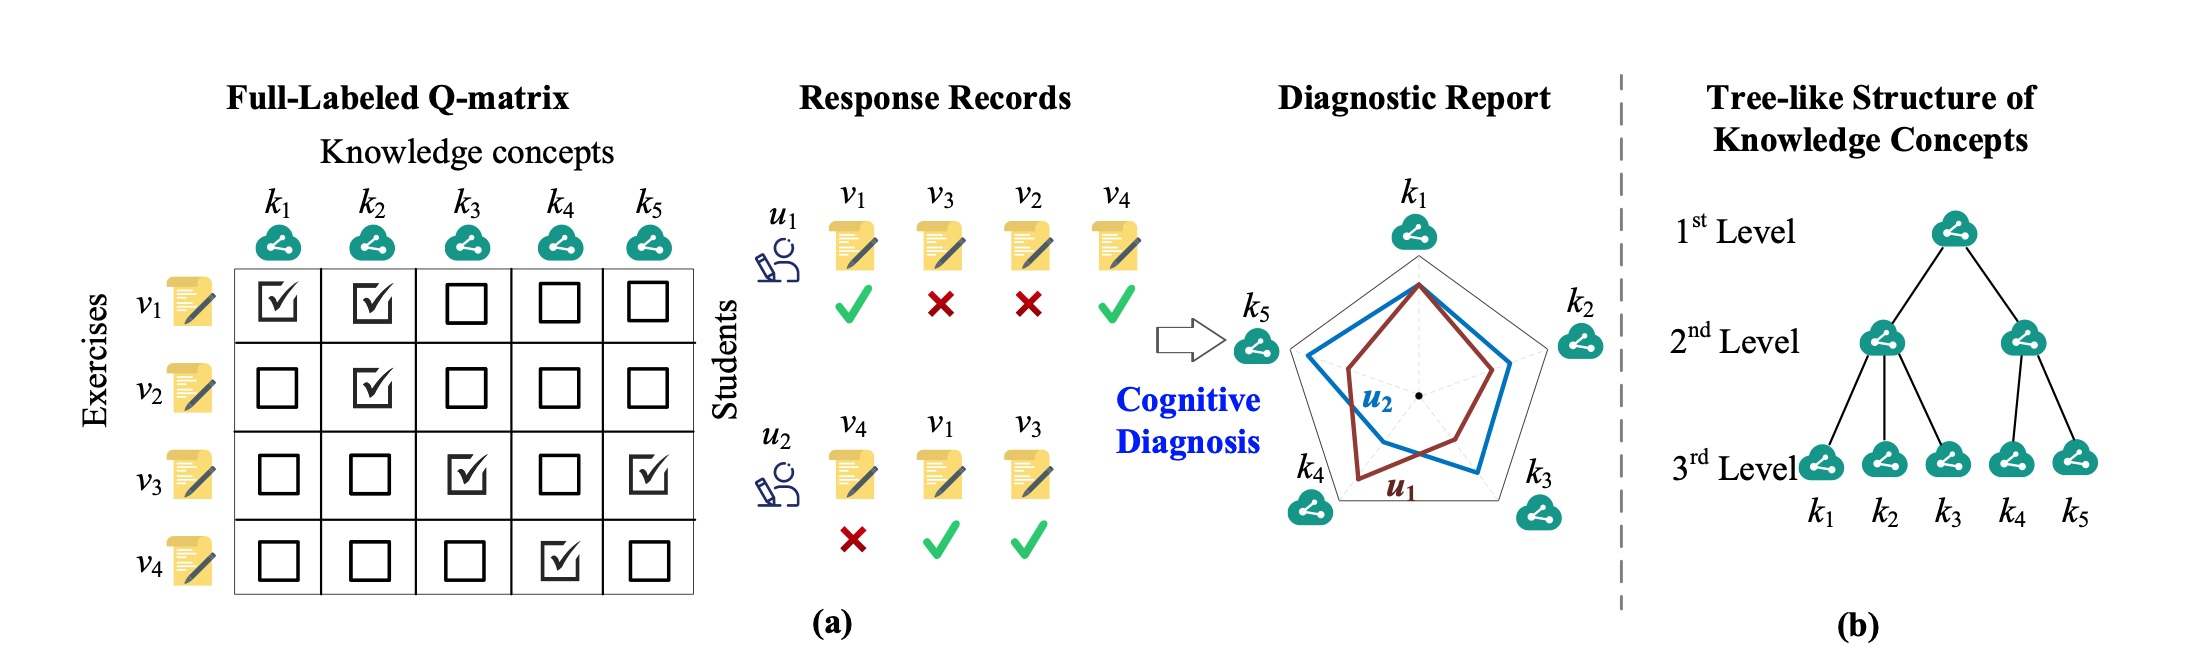
\includegraphics[width=\linewidth]{cd_example.png}
    \caption*{CD 任务流程示例,引自\citet{chen2024disentangling}。(a) 展示了使用专家注释的完全标注的 Q-矩阵来进行认知诊断的例子。(b) 为该过程依赖的概念的树状结构,与Q-矩阵比可以以较低成本完成标注。}
    \caption{认知诊断过程示例}
    \label{fig:cd_example}
\end{figure}

\subsection{知识追踪与认知诊断的局限性}

知识追踪与认知诊断都是利用计算机技术和算法来建模学生的认知状态和知识掌握情况进行建模的尝试。虽然已经取得了比较好的效果,但是二者仍然存在着不少局限性,很难广泛应用到教学场景中。

首先,两种方法中判断学生是否会做一道题,都是记录学生做题结果的“对与错”。这种方法并不能非常精确地判断学生是否真正理解了知识点、是否真正会做这道题,只能判断学生是否得到了正确答案,哪怕是学生刚好猜对的。这种方法只适用于选择题、判断题等解题过程比较简单、能够通过正误来准确定位到学生具体欠缺的能力或知识的题目类型,对于解答题就束手无策了,一些开放性题目如填空题和作文,也无法有效处理。其次,两种方法都是基于固定的题库和固定的知识点划分。这种方法无法适应学生的个性化需求,也无法适应教学内容的多样性。基于常见 KT 算法的个性化教学只能在题库里面选择合适的题目,而无法根据学生的实际需求生成新的题目或引入题库外的题目,实现真正的个性化教学;而由于 CD 算法的效果非常依赖对题目的标注,基于 CD 的个性化教学在引入新的题目的时候,需要人类教师标注对应的 Q-矩阵,成本较高。虽然目前有一些新的研究可以通过学习学生解题历史记录和少量(10\%-20\%)打了标签的题目,自动地对其他题目所考察的知识点和难度进行标注\cite{chen2024disentangling},但是这种方法仍然离不开人类专家的标注,且标注的成本仍然较高。

最重要的是,KT 和 CD 的方法也不能跟踪学生具体的解题过程和思路,无法进行更细粒度的分析。例如对于常见的数学解答题而言,解答的过程往往需要很多步推理、综合运用了一系列数学知识和能力。对于这类问题,学生的解题过程和思路往往比答案更重要,因为仅凭结果的正误无法推断出发生错误的步骤,更不能定位错误的根本原因到学生哪一知识的掌握比较薄弱。但 KT 和 CD 无法对这些信息进行有效的提取和分析。要想有效分析解答题的解题过程对学生能力的体现,就需要借助新的方法和工具了。


\section{认知过程的建模}

在 KT、CD 等通过学生历史做题的正误来建模学生的知识掌握情况的方法不同,认知过程的建模则是通过对学生的解题过程进行建模,用来解释大脑的认知结构以及解决问题的认知过程背后的内部知识表示机制。认知过程的建模是一种更加细粒度的建模方法,可以帮助我们更好地理解学生某次解题过程内部的认知过程,从而更好地进行个性化教学。比如\citet{wang2010cognitive} 的研究,提出了一套数学的认知模型,严谨地表示和刻画人类解决问题的过程。在他们看来,解决问题是大脑的一个认知过程,它为给定的问题寻找解决方案,或找到达到给定目标的路径。当一个问题的目标被确定后,解决问题可以被视为内存空间中的搜索过程,用于查找一组解决方案目标和一组替代路径之间的关系。研究者认为这一研究可以帮助未来一代认知计算方法的发展,以及为未来能够思考、学习和感知的新型认知计算机奠定基础。这篇研究中提出的思维过程的数学模型对于本研究所要实现的目标而言过于复杂繁琐,但其方法启发了本研究中解题过程刻画方法的设计。

\begin{figure}
    \centering
    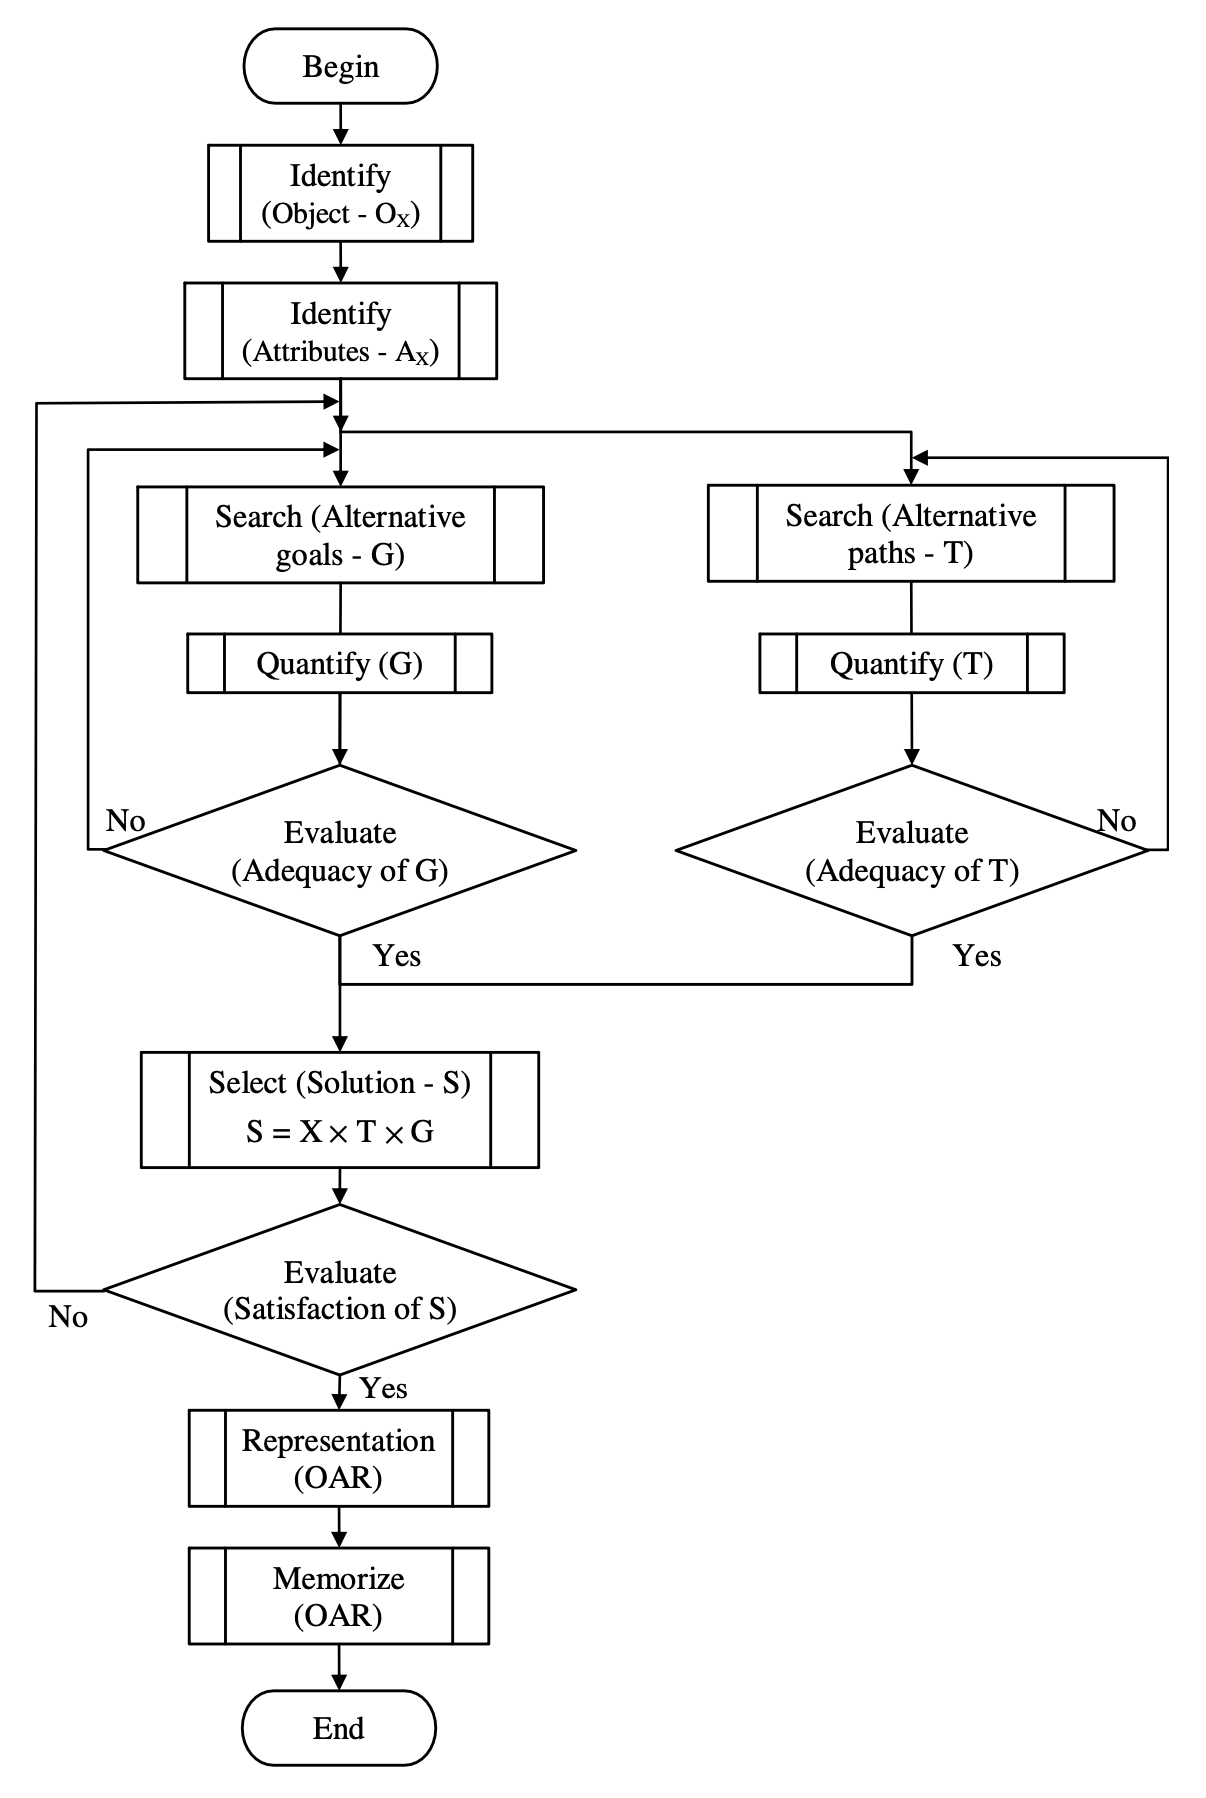
\includegraphics[width=0.5\linewidth]{cognitive_process.png}
    \caption*{一个普通的问题解决过程建模示例,引自\citet{wang2010cognitive}。其中解决问题的认知过程可以分为定义问题、搜索目标和解决路径、生成解答、选择合适的解答、表示问题解决结果这五个步骤。}
    \caption{问题解决过程建模示例}
    \label{fig:cognitive_process}
\end{figure}

\section{大语言模型}

语言模型通过对文本序列的概率进行建模,以预测给定输入后最有可能的输出序列。近年来,基于transformer架构\cite{vaswani2017attention}的语言模型在参数量和训练数据量方面不断增长,近年来不断出现更新、能力更强的大语言模型。例如LaMDA\cite{thoppilan2022lamda},PaLM\cite{anil2023palm},和 OpenAI 公司的 GPT-3 模型\cite{brown2020language}、在线大语言模型聊天服务 ChatGPT\cite{abdullah2022chatgpt},以及目前最新的支持文本和图片多模态输入的 GPT-4\cite{achiam2023gpt}。 这类被称作大语言模型 (LLM) 的大参数量模型 (千亿到万亿级别的参数量) 系统相继涌现。它们已经展示了在不需要重新训练的情况下,能够广泛适应新任务的强大泛化能力。
为了让LLM按需执行任务,用户需要精心编写自然语言指令,人们更常见地称这种输入给 LLM 的自然语言指令为提示词(prompts)。提示词可以提供少量示例(few-shot examples),也可以仅提供任务描述而不包含示例。随着人们在日常场景或工程开发上对 LLM 的使用逐渐增多,提示工程成为了与大型语言模型进行有效对话所需的一项日益重要的技能,人们也已经总结出了一系列经验上的提示词工程技术,可以提供可重复使用的解决方案\cite{white2023prompt}。LLM在多种新任务中的优异表现表明,它们在学习大规模语料的过程中,将语言中丰富的语义知识嵌入模型内部,而输入提示词的过程则可以被视作将这些知识提取出来。

LLM为人机交互带来了新的机遇\cite{bommasani2021opportunities}。它们能够处理终端用户多样化的自然语言表达,更准确地理解用户意图,使得即使缺乏专业知识的用户也能更容易地构建AI应用。此外,LLM内部蕴含的丰富知识还能作为多模态数据的粘合剂,利用其他模态的数据增强其情境理解能力,从而更好地执行任务。

总之,LLM的发展现状展示了它在自然语言处理和多模态数据集成方面的巨大潜力,通过较强的对语言的理解和生成能力,为人工智能的广泛应用提供了坚实的基础。本研究利用LLM语义理解能力和数学逻辑能力在智能教育领域的应用。通过给 LLM 提供学生的解题过程的详细内容、题目本身与标准解答图等数据,我们可以使它有效地理解学生的解题过程,将其翻译成我们规定好的结构化的数据结构,对学生认知进行建模,并以自然语言输出解题报告进行个性化的辅导。

\section{LLM 在教育领域的应用}

随着大语言模型的不断发展,在教育领域中,大型语言模型(LLM)的应用前景广阔且充满潜力\cite{gan2023large}。这些应用不仅能够提升教学质量,还能显著改善学生的学习体验。

首先,LLM能够根据学生的学习需求和兴趣,提供个性化的学习内容和推荐,从而帮助学生更有效地学习和成长。通过分析学生的学习数据和行为模式,LLM可以设计出独特的学习路径和资源,满足每个学生的个性化需求。对于特定的学科(比如英语),大模型也可以根据需求生成高质量的练习题,使得学生的练习不再受限于固定的题库。

此外,LLM作为教师的辅助工具,能够为教师提供智能教学支持平台。这些平台可以生成内容和建议,帮助教师设计教学活动、监控学生的学习进度,并提供个性化的教学支持。教师可以利用LLM生成的内容和建议,进行更有针对性的教学,从而提高教学效率和效果。

在教育评估方面,LLM也展现了巨大的潜力。通过自动分析学生的作业、考试等学习数据,LLM能够提供关于学生学习进展的评估和反馈。这不仅提高了评估的效率,还能为教师和学生提供及时的反馈,帮助他们及时调整教学和学习策略,从而促进学生的学习和成长。

然而,LLM在教育中的应用也面临一些挑战。首先是数据隐私和安全问题。智能教育需要收集和分析大量学生数据,这引发了对学生隐私和数据安全的担忧。因此,建立健全的数据管理和保护机制,确保学生数据的安全和合法使用,是智能教育发展的关键。其次是技术基础设施和资源的需求。智能教育的实施需要充足的技术基础设施和资源支持,包括网络连接、计算设备、教育软件等。然而,目前一些地区和学校可能面临技术条件和资源匮乏的问题,这限制了智能教育的广泛应用和推广。制定相关的法律法规,确保智能教育在带来教育效益的同时,遵循伦理原则和社会公平,是下一步推广智能教育时的重要社会议题。
% !TeX root = ../thuthesis-example.tex

\chapter{数学符号和公式}

\section{数学符号}

中文论文的数学符号默认遵循 GB/T 3102.11—1993《物理科学和技术中使用的数学符号》
\footnote{原 GB 3102.11—1993,自 2017 年 3 月 23 日起,该标准转为推荐性标准。}。
该标准参照采纳 ISO 31-11:1992 \footnote{目前已更新为 ISO 80000-2:2019。},
但是与 \TeX{} 默认的美国数学学会(AMS)的符号习惯有所区别。
具体地来说主要有以下差异:
\begin{enumerate}
  \item 大写希腊字母默认为斜体,如
    \begin{equation*}
      \Gamma \Delta \Theta \Lambda \Xi \Pi \Sigma \Upsilon \Phi \Psi \Omega.
    \end{equation*}
    注意有限增量符号 $\increment$ 固定使用正体,模板提供了 \cs{increment} 命令。
  \item 小于等于号和大于等于号使用倾斜的字形 $\le$、$\ge$。
  \item 积分号使用正体,比如 $\int$、$\oint$。
  \item
    偏微分符号 $\partial$ 使用正体。
  \item
    省略号 \cs{dots} 按照中文的习惯固定居中,比如
    \begin{equation*}
      1, 2, \dots, n \quad 1 + 2 + \dots + n.
    \end{equation*}
  \item
    实部 $\Re$ 和虚部 $\Im$ 的字体使用罗马体。
\end{enumerate}

以上数学符号样式的差异可以在模板中统一设置。
另外国标还有一些与 AMS 不同的符号使用习惯,需要用户在写作时进行处理:
\begin{enumerate}
  \item 数学常数和特殊函数名用正体,如
    \begin{equation*}
      \uppi = 3.14\dots; \quad
      \symup{i}^2 = -1; \quad
      \symup{e} = \lim_{n \to \infty} \left( 1 + \frac{1}{n} \right)^n.
    \end{equation*}
  \item 微分号使用正体,比如 $\dif y / \dif x$。
  \item 向量、矩阵和张量用粗斜体(\cs{symbf}),如 $\symbf{x}$、$\symbf{\Sigma}$、$\symbfsf{T}$。
  \item 自然对数用 $\ln x$ 不用 $\log x$。
\end{enumerate}


英文论文的数学符号使用 \TeX{} 默认的样式。
如果有必要,也可以通过设置 \verb|math-style| 选择数学符号样式。

关于量和单位推荐使用
\href{http://mirrors.ctan.org/macros/latex/contrib/siunitx/siunitx.pdf}{\pkg{siunitx}}
宏包,
可以方便地处理希腊字母以及数字与单位之间的空白,
比如:
\SI{6.4e6}{m},
\SI{9}{\micro\meter},
\si{kg.m.s^{-1}},
\SIrange{10}{20}{\degreeCelsius}。



\section{数学公式}

数学公式可以使用 \env{equation} 和 \env{equation*} 环境。
注意数学公式的引用应前后带括号,通常使用 \cs{eqref} 命令,比如式\eqref{eq:example}。
\begin{equation}
  \frac{1}{2 \uppi \symup{i}} \int_\gamma f = \sum_{k=1}^m n(\gamma; a_k) \mathscr{R}(f; a_k).
  \label{eq:example}
\end{equation}

多行公式尽可能在“=”处对齐,推荐使用 \env{align} 环境。
\begin{align}
  a & = b + c + d + e \\
    & = f + g
\end{align}



\section{数学定理}

定理环境的格式可以使用 \pkg{amsthm} 或者 \pkg{ntheorem} 宏包配置。
用户在导言区载入这两者之一后,模板会自动配置 \env{theorem}、\env{proof} 等环境。

\begin{theorem}[Lindeberg--Lévy 中心极限定理]
  设随机变量 $X_1, X_2, \dots, X_n$ 独立同分布, 且具有期望 $\mu$ 和有限的方差 $\sigma^2 \ne 0$,
  记 $\bar{X}_n = \frac{1}{n} \sum_{i+1}^n X_i$,则
  \begin{equation}
    \lim_{n \to \infty} P \left(\frac{\sqrt{n} \left( \bar{X}_n - \mu \right)}{\sigma} \le z \right) = \Phi(z),
  \end{equation}
  其中 $\Phi(z)$ 是标准正态分布的分布函数。
\end{theorem}
\begin{proof}
  Trivial.
\end{proof}

同时模板还提供了 \env{assumption}、\env{definition}、\env{proposition}、
\env{lemma}、\env{theorem}、\env{axiom}、\env{corollary}、\env{exercise}、
\env{example}、\env{remar}、\env{problem}、\env{conjecture} 这些相关的环境。

% !TeX root = ../__ylc_main.tex

\chapter{引用文献的标注}

模板支持 BibTeX 和 BibLaTeX 两种方式处理参考文献。
下文主要介绍 BibTeX 配合 \pkg{natbib} 宏包的主要使用方法。


\section{顺序编码制}

在顺序编码制下,默认的 \cs{cite} 命令同 \cs{citep} 一样,序号置于方括号中,
引文页码会放在括号外。
统一处引用的连续序号会自动用短横线连接。

\thusetup{
  cite-style = super,
}
\noindent
\begin{tabular}{l@{\quad$\Rightarrow$\quad}l}
  \verb|\cite{zhangkun1994}|               & \cite{zhangkun1994}               \\
  \verb|\citet{zhangkun1994}|              & \citet{zhangkun1994}              \\
  \verb|\citep{zhangkun1994}|              & \citep{zhangkun1994}              \\
  \verb|\cite[42]{zhangkun1994}|           & \cite[42]{zhangkun1994}           \\
  \verb|\cite{zhangkun1994,zhukezhen1973}| & \cite{zhangkun1994,zhukezhen1973} \\
\end{tabular}


也可以取消上标格式,将数字序号作为文字的一部分。
建议全文统一使用相同的格式。

\thusetup{
  cite-style = inline,
}
\noindent
\begin{tabular}{l@{\quad$\Rightarrow$\quad}l}
  \verb|\cite{zhangkun1994}|               & \cite{zhangkun1994}               \\
  \verb|\citet{zhangkun1994}|              & \citet{zhangkun1994}              \\
  \verb|\citep{zhangkun1994}|              & \citep{zhangkun1994}              \\
  \verb|\cite[42]{zhangkun1994}|           & \cite[42]{zhangkun1994}           \\
  \verb|\cite{zhangkun1994,zhukezhen1973}| & \cite{zhangkun1994,zhukezhen1973} \\
\end{tabular}



\section{著者-出版年制}

著者-出版年制下的 \cs{cite} 跟 \cs{citet} 一样。

\thusetup{
  cite-style = author-year,
}
\noindent
\begin{tabular}{@{}l@{$\Rightarrow$}l@{}}
  \verb|\cite{zhangkun1994}|                & \cite{zhangkun1994}                \\
  \verb|\citet{zhangkun1994}|               & \citet{zhangkun1994}               \\
  \verb|\citep{zhangkun1994}|               & \citep{zhangkun1994}               \\
  \verb|\cite[42]{zhangkun1994}|            & \cite[42]{zhangkun1994}            \\
  \verb|\citep{zhangkun1994,zhukezhen1973}| & \citep{zhangkun1994,zhukezhen1973} \\
\end{tabular}

\vskip 2ex
\thusetup{
  cite-style = super,
}
注意,引文参考文献的每条都要在正文中标注
\cite{zhangkun1994,zhukezhen1973,dupont1974bone,zhengkaiqing1987,%
  jiangxizhou1980,jianduju1994,merkt1995rotational,mellinger1996laser,%
  bixon1996dynamics,mahui1995,carlson1981two,taylor1983scanning,%
  taylor1981study,shimizu1983laser,atkinson1982experimental,%
  kusch1975perturbations,guangxi1993,huosini1989guwu,wangfuzhi1865songlun,%
  zhaoyaodong1998xinshidai,biaozhunhua2002tushu,chubanzhuanye2004,%
  who1970factors,peebles2001probability,baishunong1998zhiwu,%
  weinstein1974pathogenic,hanjiren1985lun,dizhi1936dizhi,%
  tushuguan1957tushuguanxue,aaas1883science,fugang2000fengsha,%
  xiaoyu2001chubanye,oclc2000about,scitor2000project%
}。

% !TeX root = ../__ylc_main.tex

\chapter{评估分析}

为了衡量本研究提出的解题过程评估系统的有效性,我们在真实教学场景中采集学生的解题数据,并请教师以及人类专家对其进行分析。本章节将介绍我们的实验设计、流程和实验分析。

\section{实验设计与流程}

\subsection{参与者}

我们在西宁二十一中实地考察期间组织了用户实验,实验参与者包括两名高中数学老师以及老师帮助我们选出的20位高二学生。学生的年龄在16-18岁之间,数学水平大致能够反映班级中的分布。

\subsection{实验流程}

我们选用当天数学作业中的一道解答题作为实验题目,要求学生现场作答,不限时。我们要求被试在做题的过程中需要尽可能边思考边说 (也称作 think aloud),就像平常练习一样自然地解题,但是尽可能把解题过程中的真实想法和思路说出来。测试所用题目如下:

\begin{quote}
    \begin{description}
        \item[实验题目] 已知函数 $f(x) = ax^2 + b \ln x$ 在 $x=1$ 处有极值 $\frac{1}{2}$.

        (1) 求 $a, b$ 的值;

        (2) 求出 $f(x)$ 的单调区间,并求极值.

    \end{description}
\end{quote}

考虑到后期实际落地的成本,不太可能位每一个学生都配备手写板和智能平板,本次实验仅记录音频和图片信息,探究我们的系统基于这些信息进行分析的效果。学生在解答过程中,实验人员使用手机对学生的解题过程进行录音记录,并在解题完成后对答题纸拍照留存。学生完成解答后,我们将数据汇总并逐一进行解题过程的思路建模和错因分析。

在20份学生解答中,我们选取了字迹较为工整、数据质量较高且具有代表性的 8 份解答过程,将解题过程评估系统给出的分析报告进行汇总,交给老师对这些解答过程的分析结果依次进行评分。共有 5 位被试对系统的输出进行了评分,包括两位老师和 3 位 校内被试。此外我们还通过一个简短的访谈请两位老师对系统使用体验进行总体上的评价。

\subsection{评价方式}

对于一份学生解题过程,系统给出的解题分析报告的例子如图\ref{fig:analysis_example}。为了衡量评判的准确程度,老师需要判断系统对于每一步正确性判断是否正确,以及根本错因分析是否有冗余或缺失。

在随后的访谈部分,我们请教师从实际应用角度衡量我们系统能够有多大帮助。具体来讲,我们请老师思考对于“收齐全班的作业,在批改的过程中分析每位学生的错误点,并对全班的知识掌握情况有所了解,从而指导第二天根据作业情况进行针对性教学”这一任务,考虑以下两种方法来实现的情景,并从多个维度进行对比打分:

\begin{enumerate}
    \item 按传统方式手动批改,在答卷上批注,并总结全班掌握情况;
    \item 使用我们的系统,直接浏览每位学生的解题分析报告以及全班的统计数据。如有必要也可以直接查看答卷。
\end{enumerate}

我们使用基于 NASA-TLX \footnote{NASA Task Load Index (NASA-TLX) 是一个客观的、多维度的任务负荷评估方式,在人机交互研究中广泛使用。}的问卷来衡量老师对于两种完成任务方法分别的认知负荷,要求老师对以下命题按照 1 - 7 的分数标准进行评分(1 代表程度最低,7 代表程度最高):

\begin{itemize}
    \item 脑力需求:任务需要多少心理和知觉活动(如思考、决定、计算、记忆等)
    \item 体力需求:任务需要多少体力活动(实际进行思考之外的活动)
    \item 时间需求:时间的压力有多大(如时间限制、任务速度等)
    \item 自我表现:对自己执行任务的表现是否满意,完成任务的成功程度
    \item 努力程度:为了完成任务需要付出多少努力(工作量)
    \item 挫折感:在完成任务过程中感受到多少压力、沮丧和挫折感
\end{itemize}

随后我们要求老师从以下方面对总体使用体验进行评价,同样按照 1 - 7 的分数标准进行评分(1 代表完全不认同,7 代表非常认同):

\begin{itemize}
    \item 目前的解题分析报告是否足够清晰简洁、易于理解?
    \item 总体而言,您在多大程度上相信我们系统给出的判断?
    \item 未来如果自动判作业系统开发成熟,您多大程度上愿意使用它来辅助教学?
\end{itemize}

\section{实验结果分析}

\subsection{系统准确性}

经过专家评估,在上述实验中选用的 8 份解答过程中,系统对于每一步骤学生解答的正确性判断准确率平均为 98.25\%;根本错误点分析准确性则稍微弱一点,对于每一份解答过程的分析报告中,根本错因分析平均有 31\% 的概率发生冗余,以及 18\% 的概率发生遗漏。在实际应用中,系统的准确性表现得较为稳定,虽然准确性仍有待提高,对于大部分学生的解答过程都能给出对于老师的教学有参考价值的分析报告。

\subsection{访谈结论}

在访谈部分,我们请老师对于两种完成任务方法的认知负荷进行评分,结果如表\ref{tab:nasa-tlx}所示(多位被试的打分取均值)。从表中可以看出,老师在使用我们的系统进行任务的认知负荷要明显低于传统手动批改的方式,具体体现在对于脑力、体力、时间的需求以及努力程度上,使用我们系统所需要付出的都更低。这是因为老师可以省去逐一批改学生的作业并记忆常见的错误原因与易错点,直接参考系统给出的对于班级整体批改后得到的统计数据。在自我表现和挫折感这两个维度上,老师对于使用我们系统的评价都略优于传统手动批改的方式。这说明我们的系统在实际应用中能够有效地减轻老师的工作负担。

\begin{table}
    \centering
    \caption{认知负荷评分结果}
    \label{tab:nasa-tlx}
    \begin{tabular}{c|cccccc}
        \toprule
        & \textbf{脑力需求} & \textbf{体力需求} & \textbf{时间需求} & \textbf{自我表现} & \textbf{努力程度} & \textbf{挫折感} \\
        \midrule
        \textbf{传统手动批改} & 6.5 & 6 & 6.5 & 4.5 & 6.5 & 7 \\
        \textbf{使用我们系统} & 2 & 1.5 & 2 & 5.5 & 2 & 3.5 \\
        \bottomrule
    \end{tabular}
\end{table}

总体来讲老师认为我们的系统给出的分析报告比较清晰易懂(5.5 分),并且在一定程度上相信系统给出的判断(5 分)。在未来如果自动判作业系统开发成熟,老师愿意使用它来辅助教学的意愿也较高(6.0 分)。

老师特别表达了希望看到全班的错误点和错因统计结果的意愿,因为对于老师的实际教学来说,全班的知识掌握情况对于通过大班授课来进行针对性指导是更为重要的。基于目前每道题的自动批改结果,我们已经能够一定程度上达到这一目标。对于每一道题,我们可以整理所有答卷中有错误的数量;可以统计每个错误点出现的次数并进行排序,从而了解到全班的易错点有哪些;还可以整理未掌握人数较多的知识点进行针对性讲解。我们访谈的老师认为这一点在实际应用中是非常有意义的。




% 其他部分
\backmatter

% 参考文献
\bibliography{ref/refs}  % 参考文献使用 BibTeX 编译
% \printbibliography       % 参考文献使用 BibLaTeX 编译

% 附录
% 本科生需要将附录放到声明之后,个人简历之前
\appendix
% % !TeX root = ../thuthesis-example.tex

\begin{survey}
\label{cha:survey}

\title{Title of the Survey}
\maketitle


\tableofcontents


本科生的外文资料调研阅读报告。


\section{Figures and Tables}

\subsection{Figures}

An example figure in appendix (Figure~\ref{fig:appendix-survey-figure}).

\begin{figure}
  \centering
  \includegraphics[width=0.6\linewidth]{example-image-a.pdf}
  \caption{Example figure in appendix}
  \label{fig:appendix-survey-figure}
\end{figure}


\subsection{Tables}

An example table in appendix (Table~\ref{tab:appendix-survey-table}).

\begin{table}
  \centering
  \caption{Example table in appendix}
  \begin{tabular}{ll}
    \toprule
    File name       & Description                                         \\
    \midrule
    thuthesis.dtx   & The source file including documentation and comments \\
    thuthesis.cls   & The template file                                   \\
    thuthesis-*.bst & BibTeX styles                                       \\
    thuthesis-*.bbx & BibLaTeX styles for bibliographies                  \\
    thuthesis-*.cbx & BibLaTeX styles for citations                       \\
    \bottomrule
  \end{tabular}
  \label{tab:appendix-survey-table}
\end{table}


\section{Equations}

An example equation in appendix (Equation~\eqref{eq:appendix-survey-equation}).
\begin{equation}
  \frac{1}{2 \uppi \symup{i}} \int_\gamma f = \sum_{k=1}^m n(\gamma; a_k) \mathscr{R}(f; a_k)
  \label{eq:appendix-survey-equation}
\end{equation}


\section{Citations}

Example\cite{dupont1974bone} citations\cite{merkt1995rotational} in appendix
\cite{dupont1974bone,merkt1995rotational}.


% 默认使用正文的参考文献样式;
% 如果使用 BibTeX,可以切换为其他兼容 natbib 的 BibTeX 样式。
\bibliographystyle{unsrtnat}
% \bibliographystyle{IEEEtranN}

% 默认使用正文的参考文献 .bib 数据库;
% 如果使用 BibTeX,可以改为指定数据库,如 \bibliography{ref/refs}。
\printbibliography

\end{survey}
       % 本科生:外文资料的调研阅读报告
% % !TeX root = ../thuthesis-example.tex

\begin{translation}
\label{cha:translation}

\title{书面翻译题目}
\maketitle

\tableofcontents


本科生的外文资料书面翻译。


\section{图表示例}

\subsection{图}

附录中的图片示例(图~\ref{fig:appendix-translation-figure})。

\begin{figure}
  \centering
  \includegraphics[width=0.6\linewidth]{example-image-a.pdf}
  \caption{附录中的图片示例}
  \label{fig:appendix-translation-figure}
\end{figure}


\subsection{表格}

附录中的表格示例(表~\ref{tab:appendix-translation-table})。

\begin{table}
  \centering
  \caption{附录中的表格示例}
  \begin{tabular}{ll}
    \toprule
    文件名          & 描述                         \\
    \midrule
    thuthesis.dtx   & 模板的源文件,包括文档和注释 \\
    thuthesis.cls   & 模板文件                     \\
    thuthesis-*.bst & BibTeX 参考文献表样式文件    \\
    thuthesis-*.bbx & BibLaTeX 参考文献表样式文件  \\
    thuthesis-*.cbx & BibLaTeX 引用样式文件        \\
    \bottomrule
  \end{tabular}
  \label{tab:appendix-translation-table}
\end{table}


\section{数学公式}

附录中的数学公式示例(公式\eqref{eq:appendix-translation-equation})。
\begin{equation}
  \frac{1}{2 \uppi \symup{i}} \int_\gamma f = \sum_{k=1}^m n(\gamma; a_k) \mathscr{R}(f; a_k)
  \label{eq:appendix-translation-equation}
\end{equation}


\section{文献引用}

附录\cite{dupont1974bone}中的参考文献引用\cite{merkt1995rotational}示例
\cite{dupont1974bone,merkt1995rotational}。


\appendix

\section{附录}

附录的内容。


% 书面翻译的参考文献
% 默认使用正文的参考文献样式;
% 如果使用 BibTeX,可以切换为其他兼容 natbib 的 BibTeX 样式。
\bibliographystyle{unsrtnat}
% \bibliographystyle{IEEEtranN}

% 默认使用正文的参考文献 .bib 数据库;
% 如果使用 BibTeX,可以改为指定数据库,如 \bibliography{ref/refs}。
\printbibliography

% 书面翻译对应的原文索引
\begin{translation-index}
  \nocite{mellinger1996laser}
  \nocite{bixon1996dynamics}
  \nocite{carlson1981two}
  \bibliographystyle{unsrtnat}
  \printbibliography
\end{translation-index}

\end{translation}
  % 本科生:外文资料的书面翻译
% !TeX root = ../thuthesis-example.tex

\chapter{补充内容}

附录是与论文内容密切相关、但编入正文又影响整篇论文编排的条理和逻辑性的资料,例如某些重要的数据表格、计算程序、统计表等,是论文主体的补充内容,可根据需要设置。

附录中的图、表、数学表达式、参考文献等另行编序号,与正文分开,一律用阿拉伯数字编码,
但在数码前冠以附录的序号,例如“图~\ref{fig:appendix-figure}”,
“表~\ref{tab:appendix-table}”,“式\eqref{eq:appendix-equation}”等。


\section{插图}

% 附录中的插图示例(图~\ref{fig:appendix-figure})。

\begin{figure}
  \centering
  \includegraphics[width=0.6\linewidth]{example-image-a.pdf}
  \caption{附录中的图片示例}
  \label{fig:appendix-figure}
\end{figure}


\section{表格}

% 附录中的表格示例(表~\ref{tab:appendix-table})。

\begin{table}
  \centering
  \caption{附录中的表格示例}
  \begin{tabular}{ll}
    \toprule
    文件名          & 描述                         \\
    \midrule
    thuthesis.dtx   & 模板的源文件,包括文档和注释 \\
    thuthesis.cls   & 模板文件                     \\
    thuthesis-*.bst & BibTeX 参考文献表样式文件    \\
    thuthesis-*.bbx & BibLaTeX 参考文献表样式文件  \\
    thuthesis-*.cbx & BibLaTeX 引用样式文件        \\
    \bottomrule
  \end{tabular}
  \label{tab:appendix-table}
\end{table}


\section{数学表达式}

% 附录中的数学表达式示例(式\eqref{eq:appendix-equation})。
\begin{equation}
  \frac{1}{2 \uppi \symup{i}} \int_\gamma f = \sum_{k=1}^m n(\gamma; a_k) \mathscr{R}(f; a_k)
  \label{eq:appendix-equation}
\end{equation}


\section{文献引用}

附录\cite{dupont1974bone}中的参考文献引用\cite{zhengkaiqing1987}示例
\cite{dupont1974bone,zhengkaiqing1987}。

\printbibliography


% 致谢
% !TeX root = ../__ylc_main.tex

\begin{acknowledgements}
  衷心感谢导师×××教授和物理系××副教授对本人的精心指导。他们的言传身教将使我终生受益。

  在美国麻省理工学院化学系进行九个月的合作研究期间,承蒙 Robert Field 教授热心指导与帮助,不胜感激。

  感谢×××××实验室主任×××教授,以及实验室全体老师和同窗们学的热情帮助和支持!

  本课题承蒙国家自然科学基金资助,特此致谢。
\end{acknowledgements}


% 声明
% 本科生开题报告不需要
\statement
% 将签字扫描后的声明文件 scan-statement.pdf 替换原始页面
% \statement[file=scan-statement.pdf]
% 本科生编译生成的声明页默认不加页脚,插入扫描版时再补上;
% 研究生编译生成时有页眉页脚,插入扫描版时不再重复。
% 也可以手动控制是否加页眉页脚
% \statement[page-style=empty]
% \statement[file=scan-statement.pdf, page-style=plain]

% 个人简历、在学期间完成的相关学术成果
% 本科生可以附个人简历,也可以不附个人简历
% % !TeX root = ../thuthesis-example.tex

\begin{resume}

  \section*{个人简历}

  197× 年 ×× 月 ×× 日出生于四川××县。

  1992 年 9 月考入××大学化学系××化学专业,1996 年 7 月本科毕业并获得理学学士学位。

  1996 年 9 月免试进入清华大学化学系攻读××化学博士至今。


  \section*{在学期间完成的相关学术成果}

  \subsection*{学术论文}

  \begin{achievements}
    \item Yang Y, Ren T L, Zhang L T, et al. Miniature microphone with silicon-based ferroelectric thin films[J]. Integrated Ferroelectrics, 2003, 52:229-235.
    \item 杨轶, 张宁欣, 任天令, 等. 硅基铁电微声学器件中薄膜残余应力的研究[J]. 中国机械工程, 2005, 16(14):1289-1291.
    \item 杨轶, 张宁欣, 任天令, 等. 集成铁电器件中的关键工艺研究[J]. 仪器仪表学报, 2003, 24(S4):192-193.
    \item Yang Y, Ren T L, Zhu Y P, et al. PMUTs for handwriting recognition. In press[J]. (已被Integrated Ferroelectrics录用)
  \end{achievements}


  \subsection*{专利}

  \begin{achievements}
    \item 任天令, 杨轶, 朱一平, 等. 硅基铁电微声学传感器畴极化区域控制和电极连接的方法: 中国, CN1602118A[P]. 2005-03-30.
    \item Ren T L, Yang Y, Zhu Y P, et al. Piezoelectric micro acoustic sensor based on ferroelectric materials: USA, No.11/215, 102[P]. (美国发明专利申请号.)
  \end{achievements}

\end{resume}


% 指导教师/指导小组评语
% 本科生不需要
% % !TeX root = ../thuthesis-example.tex

\begin{comments}
% \begin{comments}[name = {指导小组评语}]
% \begin{comments}[name = {Comments from Thesis Supervisor}]
% \begin{comments}[name = {Comments from Thesis Supervision Committee}]

  论文提出了……

\end{comments}


% 答辩委员会决议书
% 本科生不需要
% % !TeX root = ../thuthesis-example.tex

\begin{resolution}

  论文提出了……

  论文取得的主要创新性成果包括:

  1. ……

  2. ……

  3. ……

  论文工作表明作者在×××××具有×××××知识,具有××××能力,论文××××,答辩××××。

  答辩委员会表决,(×票/一致)同意通过论文答辩,并建议授予×××(姓名)×××(门类)学博士/硕士学位。

\end{resolution}


% 本科生的综合论文训练记录表(扫描版)
% \record{file=scan-record.pdf}

\end{document}
